% Standalone title graphic for the slides.
% A schematic of the L3902 boot trampoline — three boxes, three jumps,
% drawn in TikZ. Compiled to title-graphic.pdf and embedded in slides.tex.

\documentclass[tikz,border=4pt]{standalone}
\usepackage{tikz}
\usetikzlibrary{positioning,arrows.meta,backgrounds,fit,calc}

\begin{document}
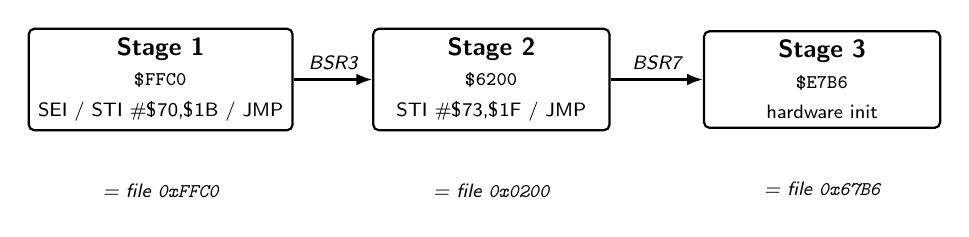
\begin{tikzpicture}[
  font=\sffamily\small,
  stage/.style={draw,thick,rounded corners=2pt,minimum width=3.0cm,minimum height=1.0cm,align=center,fill=white},
  arrow/.style={-{Latex[length=2mm]},thick},
  label/.style={font=\sffamily\scriptsize\itshape},
]

  % Three stages of the boot trampoline.
  \node[stage] (s1) at (0,0)
    {\textbf{Stage 1} \\ \scriptsize \texttt{\$FFC0} \\ \scriptsize SEI / STI \#\$70,\$1B / JMP};
  \node[stage] (s2) at (4.2,0)
    {\textbf{Stage 2} \\ \scriptsize \texttt{\$6200} \\ \scriptsize STI \#\$73,\$1F / JMP};
  \node[stage] (s3) at (8.4,0)
    {\textbf{Stage 3} \\ \scriptsize \texttt{\$E7B6} \\ \scriptsize hardware init};

  \draw[arrow] (s1) -- (s2) node[midway,above,label] {BSR3};
  \draw[arrow] (s2) -- (s3) node[midway,above,label] {BSR7};

  % File-offset annotation underneath.
  \node[label,below=0.55cm of s1] {= file \texttt{0xFFC0}};
  \node[label,below=0.55cm of s2] {= file \texttt{0x0200}};
  \node[label,below=0.55cm of s3] {= file \texttt{0x67B6}};

\end{tikzpicture}
\end{document}
